% ICCIES 2027 submission -- Springer CCIS (LNCS/LNAI style), 12--15 pages.
% Build:  latexmk -pdf main.tex     (or: pdflatex main; bibtex main; pdflatex main; pdflatex main)
\documentclass[runningheads]{llncs}
\usepackage[T1]{fontenc}
\usepackage{newtxtext}
\usepackage[varvw]{newtxmath}
\usepackage{graphicx}
\usepackage{marvosym} % \Letter symbol for the corresponding author
\usepackage{booktabs}
\usepackage{multirow}
\usepackage{array}
\usepackage{tikz}
\usetikzlibrary{positioning,arrows.meta,fit,backgrounds}
\usepackage[hidelinks]{hyperref}
\usepackage{color}
\renewcommand\UrlFont{\color{blue}\rmfamily}
\urlstyle{rm}
% \Description is defined by llncs v2.25; keep the file compiling with older class versions.
\providecommand{\Description}[1]{}

% ---------------------------------------------------------------------------
% RQ3 uses the column "Nguồn sinh câu hỏi" (Graph / Codebase) of the survey export.
\newif\ifrqthree \rqthreetrue
\newcommand{\TBD}{\textbf{\color{red}TBD}}
% ---------------------------------------------------------------------------

\begin{document}

\title{Do Students Agree with LLM Feedback on Their Own Code? A Within-Subject Study of Four Feedback Formats in Software Project Courses}
\titlerunning{Student Agreement with LLM Feedback on Their Own Code}

% Names are written given-name first without diacritics, as Springer's metadata expects.
% Corresponding author: Phuc Thinh Do. TODO: add ORCID iDs (\orcidID{...}) if available.
\author{Phuc Sanh Nguyen \and
Song Huong Dang \and
Quang Hieu Le \and
Viet~Bao~Nguyen \and
Phuc~Thinh~Do\textsuperscript{(\Letter)}}
\authorrunning{P. S. Nguyen et al.}
\institute{FPT University, Ho Chi Minh City, Vietnam\\
\email{npsdn1906@gmail.com, dangsonghuong010405@gmail.com, lequanghieu2504@gmail.com, babluokei4@gmail.com, ThinhDP2@fe.edu.vn}}

\maketitle

\begin{abstract}
Large language models (LLMs) can comment on student work at a scale no teaching team can match, but feedback only helps if students accept it. We study this in a setting that has received little attention: comprehension questions that an AI system generates from the source code of each student's own team project. Our platform, PACE, analyses a repository, asks each student four scenario questions about business rules in that code, and returns LLM feedback on every answer in one of four formats---Sandwich, Rubric, Explainable, and a two-model Researching ensemble---assigned by random permutation within each student. Eighty-six students in software project courses rated all 344 feedback instances they received on a 15-item instrument. Agreement was positive (4.07/5, 95\% CI [3.95, 4.19]): more than 80\% of ratings endorsed the accuracy, specificity and usefulness of the feedback, yet only 68\% expressed an intention to keep using the system and 42\% said the feedback motivated them. Perceived utility and trust predicted acceptance more strongly than perceived quality. Format effects were detectable but small (Friedman $\chi^2(3)=23.0$, $p<.001$, Kendall's $W=.09$): the two formats that end with explicit next steps, Sandwich and Researching, were rated more actionable, and Rubric feedback drew less trust. No pair of formats differed by more than $\pm0.25$ points, and acceptance itself did not vary. Questions generated from raw code and from a data-flow graph received similar agreement ($b=0.08$, $p=.22$). An intraclass correlation of .77 shows that ratings depended mostly on the student. We also find that 19\% of responses were straight-lined and that this masked the behaviour of a reverse-worded item.

\keywords{LLM-generated feedback \and Feedback acceptance \and Programming education \and Software engineering education \and Human--AI trust}
\end{abstract}

%=============================================================================
\section{Introduction}
\label{sec:intro}

Feedback is one of the strongest levers on learning, but its effect depends on what the learner does with it~\cite{hattie2007power,shute2008focus}. A comment that is correct yet ignored, or that the student does not believe, changes nothing. Research on feedback literacy therefore treats the student's uptake---making sense of a comment, judging it, and deciding to act---as part of the feedback process rather than its aftermath~\cite{carless2018feedback,winstone2017supporting}.

LLMs have made it cheap to produce written feedback on programming work, and early studies show that models such as GPT-3.5 and GPT-4 can identify many issues in student code and explain them in readable language~\cite{hellas2023exploring,kiesler2023exploring,dai2023can}. Deployed tools add guardrails so that the assistant guides rather than solves~\cite{liffiton2023codehelp}, and the computing-education community now treats generative AI as a permanent part of the course environment~\cite{denny2024computing,kasneci2023chatgpt}. Whether students \emph{accept} such feedback is a separate question. Studies comparing AI and instructor feedback report mixed results: students often find AI feedback clear and specific~\cite{zhang2024students,escalante2023ai}, yet in a randomised experiment in a Java course they judged instructor feedback more useful and improved more after receiving it~\cite{er2025assessing}, and perceptions shift once students learn that a comment came from an AI~\cite{nazaretsky2024ai}.

Two gaps motivate this paper. First, most prior work studies feedback on small, instructor-designed exercises or essays. In project-based software engineering courses, the object of assessment is a team repository that grows over a semester and that no single student fully wrote. Asking students targeted questions about \emph{their own} programs is a known way to probe comprehension~\cite{lehtinen2021lets}, but we found no study of how students respond to LLM feedback on their answers to such questions. Second, systems differ in how they \emph{present} feedback---praise--critique--praise ``sandwiches'', criterion-based rubrics, evidence-based explanations, or outputs that combine several models---and each format has a pedagogical rationale~\cite{parkes2013feedback,jonsson2007use,khosravi2022explainable,du2024improving}. We do not know whether these choices change how much students agree with the same underlying judgement.

We address these gaps with PACE (Project Assistance and Course Evaluation), a platform deployed in software project courses at FPT University. PACE analyses each team's repository, generates scenario questions about business rules implemented in it, and returns LLM feedback on every answer. Each student answered four questions and received feedback in four different formats, assigned by random permutation, then rated every feedback instance on fifteen items covering perceived quality, utility, trust, affect, and acceptance. We ask:

\begin{itemize}
  \item[\textbf{RQ1}] How do students judge the quality of LLM feedback on their answers about their own code, and how far do they accept it?
  \item[\textbf{RQ2}] Does student agreement differ across the four feedback formats?
\ifrqthree
  \item[\textbf{RQ3}] Does student agreement differ between questions generated from raw source code and questions generated from a data-flow graph of the code?
\fi
\end{itemize}

The contributions of this paper are as follows:
\begin{itemize}
  \item We describe a feedback pipeline that grounds LLM comments in the student's own repository and delivers four contrasting feedback formats under a within-subject randomised design.
  \item We report a field study with 86 students and 344 rated feedback instances. Agreement was broad, but students were more ready to accept a diagnosis than to feel motivated by it or to commit to future use, and perceived utility and trust---rather than perceived quality alone---were the strongest correlates of acceptance and continued-use intention.
  \item We show that format effects were real but small: formats that close with concrete next steps were rated more actionable, yet every pair of formats stayed within $\pm0.25$ points despite a 2.5-fold difference in length, and agreement did not differ between raw-code and graph-based questions. We also document how straight-lining distorted a reverse-worded item, which future classroom evaluations of AI feedback should plan for.
\end{itemize}


%=============================================================================
\section{Related Work}
\label{sec:related}

\subsection{LLM-Generated Feedback in Programming Education}
Hellas et al.\ analysed LLM responses to real help requests from novice programmers and found that GPT-3.5 usually identified at least one actual issue but often missed others and sometimes reported issues that did not exist~\cite{hellas2023exploring}. Kiesler et al.\ reached a similar conclusion for formative feedback on introductory exercises: the feedback was often helpful but sometimes misleading, particularly for novices who cannot tell the difference~\cite{kiesler2023exploring}. Dai et al.\ showed that ChatGPT produced more detailed feedback than human instructors and agreed closely with them when assessing the topic of students' assignments~\cite{dai2023can}. CodeHelp demonstrated that guardrails can keep an assistant from simply handing out solutions while remaining useful at course scale~\cite{liffiton2023codehelp}. These studies mostly judge feedback quality through expert coding; we study what students make of it. We also move the target from short exercises to questions about a team's production-like codebase, building on the idea of questions about learners' own code~\cite{lehtinen2021lets}.

\subsection{Student Perceptions and Acceptance of AI Feedback}
Technology-acceptance research links perceived usefulness and trust to the intention to keep using a system~\cite{davis1989perceived,venkatesh2003user}, and the human-factors literature stresses that trust should be calibrated to the system's actual reliability~\cite{lee2004trust}. People may avoid algorithms after seeing them err~\cite{dietvorst2015algorithm} or prefer algorithmic advice to human advice in other conditions~\cite{logg2019algorithm}, so neither aversion nor appreciation can be assumed. In education, Zhang et al.\ found that CS1 students rated ChatGPT feedback as consistent with formative-feedback guidelines and preferred feedback that referenced their code~\cite{zhang2024students}. Er et al.\ found that students rated instructor feedback as more useful than rubric-based AI feedback and improved more with it~\cite{er2025assessing}, and Nazaretsky et al.\ showed that students' judgements of feedback changed once its AI origin was disclosed~\cite{nazaretsky2024ai}. These results suggest that acceptance depends on more than correctness, which is why we measure trust, affect and behavioural intention alongside perceived quality.

\subsection{Feedback Formats}
Feedback formats encode different beliefs about what helps learners. The ``sandwich'' places criticism between positive comments; in a controlled study it made students feel better about feedback without improving performance~\cite{parkes2013feedback}. Rubrics make criteria explicit and can improve reliability and transparency of judgement~\cite{jonsson2007use}. Explainable-AI work in education argues that showing the evidence behind an automated judgement supports appropriate trust~\cite{khosravi2022explainable}. Multi-model setups can also help: letting several models debate improves factual accuracy~\cite{du2024improving}, and a strong model used as a judge agrees well with human preferences~\cite{zheng2023judging}. To our knowledge, no study has compared such formats within the same students; our design does so.

%=============================================================================
\section{The PACE System}
\label{sec:system}

Figure~\ref{fig:overview} summarises the pipeline. PACE consists of an ASP.NET Core (.NET~9) back end, a PostgreSQL database and a Next.js front end; the parts relevant to this study are repository analysis, question generation, and feedback generation.

\begin{figure}[t]
\centering
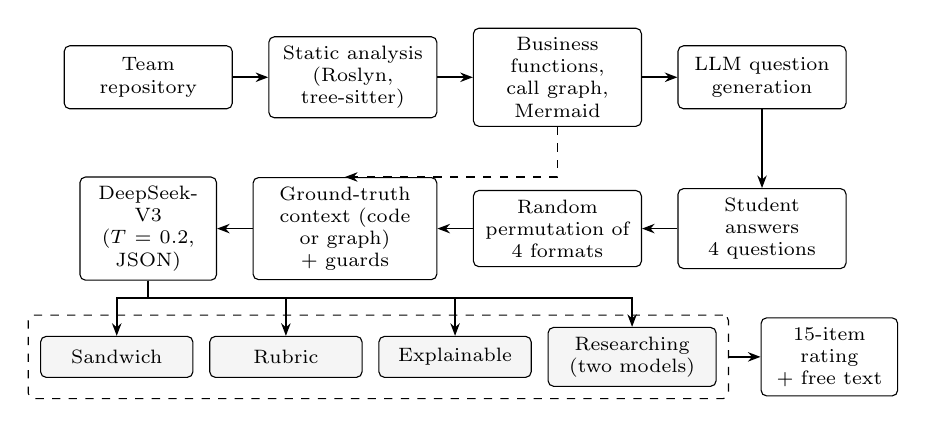
\begin{tikzpicture}[
  font=\scriptsize,
  box/.style={draw, rounded corners=2pt, align=center, minimum height=8mm, text width=19mm, fill=white},
  fmt/.style={draw, rounded corners=2pt, align=center, minimum height=5.2mm, text width=17mm, fill=black!4},
  arr/.style={-{Stealth[length=1.6mm]}, semithick},
  node distance=4mm and 4.5mm]
  \node[box] (repo) {Team\\repository};
  \node[box, right=of repo] (parse) {Static analysis\\(Roslyn, tree-sitter)};
  \node[box, right=of parse] (flow) {Business functions,\\call graph, Mermaid};
  \node[box, right=of flow] (q) {LLM question\\generation};
  \node[box, below=10mm of q] (ans) {Student answers\\4 questions};
  \node[box, left=of ans] (perm) {Random\\permutation of\\4 formats};
  \node[box, left=of perm, text width=21mm] (ctx) {Ground-truth\\context (code\\or graph) + guards};
  \node[box, left=of ctx, text width=15mm] (llm) {DeepSeek-V3\\($T=0.2$, JSON)};
  \node[fmt, below=7mm of llm, xshift=-4mm] (f1) {Sandwich};
  \node[fmt, right=2mm of f1] (f2) {Rubric};
  \node[fmt, right=2mm of f2] (f3) {Explainable};
  \node[fmt, right=2mm of f3, text width=19mm] (f4) {Researching\\(two models)};
  \begin{scope}[on background layer]\node[draw, dashed, rounded corners=2pt, inner sep=1.5mm, fit=(f1)(f4)] (fmts) {};\end{scope}
  \node[box, right=4mm of fmts, text width=15mm] (survey) {15-item rating\\+ free text};
  \draw[arr] (repo) -- (parse); \draw[arr] (parse) -- (flow); \draw[arr] (flow) -- (q);
  \draw[arr] (q) -- (ans); \draw[arr] (ans) -- (perm); \draw[arr] (perm) -- (ctx); \draw[arr] (ctx) -- (llm);
  \draw[arr] (llm.south) -- ++(0,-2.2mm) -| (f1.north);
  \draw[arr] (llm.south) -- ++(0,-2.2mm) -| (f2.north);
  \draw[arr] (llm.south) -- ++(0,-2.2mm) -| (f3.north);
  \draw[arr] (llm.south) -- ++(0,-2.2mm) -| (f4.north);
  \draw[arr] (fmts) -- (survey);
  \draw[arr, dashed] (flow.south) |- (ctx.north);
\end{tikzpicture}
\Description{Pipeline diagram. A team repository is parsed by static analysers into business functions, call graphs and Mermaid diagrams, which feed LLM question generation. Students answer four questions; the four feedback formats are randomly permuted across the answers; the evaluator receives a ground-truth context from the code and produces Sandwich, Rubric, Explainable or Researching feedback, which students rate on 15 items.}
\caption{Overview of PACE. Questions and the evaluator's ground-truth context are both derived from the student's own repository. Each student's four answers receive the four formats in a random order.}
\label{fig:overview}
\end{figure}


\subsection{Repository Analysis and Question Generation}
For each team repository, PACE clones the submitted branch and parses it with Roslyn (C\#) or tree-sitter (Java, JavaScript and TypeScript). Endpoints are grouped into \emph{business functions} (e.g., ``contract management'' or ``payment confirmation''), either from a template stored in the repository or from a draft that an instructor reviews and confirms. For every function, PACE resolves calls from each entry point and stores both the source code of the involved methods and a data-flow graph with ordered call edges, branch conditions and a Mermaid rendering.

Questions are generated per business function by GPT-6.1 Luna (temperature 0.3, structured JSON output), which receives either the raw source code or the Mermaid graph; a router selects the graph when the flow involves more than ten distinct methods and the raw code otherwise. The prompt targets scenario questions about guard conditions and failure branches, for example: \emph{``When the facility manager tries to swap the storage unit of a contract that still has an outstanding balance, how does the system respond and why is the action blocked?''} Each question is stored with a suggested answer and with the context type used to produce it. % TODO: cite prior PACE question-generation paper (if published).

\subsection{Feedback Generation}
When a student submits answers, each answer is evaluated against a \emph{ground-truth context} built from the same business function: the raw source of its methods, or its flow graph with numbered steps and conditions, following the context type of the question. The system prompt fixes an instruction hierarchy: content inside the \texttt{<student\_answer>} tag is data, never instructions; the ground-truth context and the suggested answer define correctness; the model comments and explains but does not assign an overall grade; and the output must be a single JSON object. An input guardrail rejects answers that contain prompt-injection phrases or executable payloads, and an output guardrail validates the JSON before it is stored.

The four formats differ only in the JSON schema the model must fill:
\begin{itemize}
  \item \textbf{Sandwich}: positives, constructive criticism, and next steps.
  \item \textbf{Rubric}: a list of criteria that the model names for the question (e.g., understanding of the business flow, identification of the guard condition), each with a 1--5 score and a comment.
  \item \textbf{Explainable}: a \emph{code evidence} field that cites methods, steps or conditions from the context, and a \emph{logic explanation} that relates them to the answer.
  \item \textbf{Researching}: a two-stage ensemble in which DeepSeek-V3 first inspects the answer against the code and GPT-OSS-120B (served by Groq) then writes a combined report: an overall comment, positives, criticism, next steps, code evidence, two scored criteria, and a consensus summary with pedagogical guidance.
\end{itemize}
Only Sandwich and Researching therefore contain an explicit list of next steps; Rubric and Explainable leave it to the student to infer what to change. Sandwich, Rubric and Explainable are produced by DeepSeek-V3 (\texttt{deepseek-chat}, temperature 0.2, JSON mode). If the second model in the Researching pipeline fails, the system falls back to the single-model path; in this study all 86 Researching instances were produced by the full ensemble.

The format assignment is the experimental manipulation. When a student submits $n=4$ answers, PACE shuffles the four formats and assigns one to each answer, so every student sees every format exactly once, in random order.

%=============================================================================
\section{Study Design}
\label{sec:method}

\subsection{Context and Participants}
The study took place in October 2026 in undergraduate software engineering project courses at FPT University, Vietnam. Students used PACE as a formative comprehension check on their team's repository. % TODO: state how students were recruited, whether participation was voluntary, whether it affected grades, and the consent procedure.
 The sample comprises 86 students from 28 team repositories, answering 190 distinct questions on 152 business functions. Answers were written in Vietnamese and were short, about 51 whitespace-separated tokens on average. Submissions were made between 20 and 26 October 2026.

\subsection{Instrument}
After reading each feedback instance, students rated it on fifteen statements on a five-point scale (1 = strongly disagree, 5 = strongly agree) and could add a free-text reply. The items were written in Vietnamese by the research team, drawing on formative-feedback principles~\cite{shute2008focus} and technology-acceptance constructs~\cite{davis1989perceived,venkatesh2003user,lee2004trust}. Table~\ref{tab:instrument} lists them with English translations, grouped into five a priori constructs. \textsc{Rejection} is reverse-worded.

\begin{table}[t]
\caption{Survey instrument (translated from Vietnamese). $^\dagger$Reverse-worded.}
\label{tab:instrument}
\centering\scriptsize
\setlength\tabcolsep{3pt}
\begin{tabular}{@{}p{17mm}p{20mm}p{79mm}@{}}
\toprule
Construct & Item & Statement \\
\midrule
\multirow{4}{17mm}{Perceived quality}
 & Accuracy & The AI's comment correctly identifies the problems in my answer. \\
 & Specificity & The AI points to exactly which part of my answer needs revisiting, rather than commenting in general. \\
 & Clarity & The wording and presentation of the comment are clear and unambiguous. \\
 & Transparency & I understand which academic criteria the AI used to assess my answer. \\
\midrule
\multirow{2}{17mm}{Perceived utility}
 & Usefulness & This AI tool is an effective learning assistant for my project work. \\
 & Actionability & I know exactly which technical steps to take to improve my answer. \\
\midrule
\multirow{3}{17mm}{Trust}
 & Competence & I trust the technical expertise and analytical capability of this AI. \\
 & Reliability & The AI assesses consistently and does not change its standards at random. \\
 & Fairness & The AI's assessment fairly reflects the effort and actual quality of my answer. \\
\midrule
\multirow{2}{17mm}{Affect}
 & Affect & I feel motivated to keep learning after reading the AI's comments. \\
 & Psych.\ safety & AI feedback causes less pressure than being criticised by a person. \\
\midrule
\multirow{3}{17mm}{Acceptance \& intention}
 & Acceptance & I agree with the AI's judgement of my answer's strengths and weaknesses. \\
 & Willingness & Based on this comment, I am ready to revise my answer right away. \\
 & Behav.\ intention & I intend to keep using this LLM system for feedback in future projects. \\
\midrule
Validity check & Rejection$^\dagger$ & I tend to want to refute or argue against the AI's assessment. \\
\bottomrule
\end{tabular}
\end{table}

\subsection{Data Set}
The survey export contained 344 answer records from 86 submissions, one submission per student. We screened every record on metadata only (feedback produced by an LLM call rather than a development fixture, feedback stored, all fifteen ratings present); all 344 passed, so none was excluded. Every student rated all four formats, which gives 86 complete blocks and 86 instances per format. The export also stores the context type of each question: 280 instances (157 questions) came from graph-based questions and 64 instances (33 questions, 13 repositories) from raw-code questions. Thirty-two students received at least one raw-code question, and 26 of them answered questions of both types.

\subsection{Analysis}
\paragraph{Scores.} The \emph{AI agreement index} (AAI) is the mean of the fourteen non-reversed items. Construct scores are item means. Because the reverse-worded item behaved inconsistently (Section~\ref{sec:quality}), we analyse \textsc{Rejection} separately rather than reverse-scoring it into the index~\cite{vansonderen2013ineffectiveness}.

\paragraph{Reliability and data quality.} We report Cronbach's $\alpha$~\cite{cronbach1951coefficient} and McDonald's $\omega_t$ from a one-factor solution~\cite{hayes2020use}, and flag \emph{straight-lined} responses---identical ratings on all fifteen items---following Kim et al.~\cite{kim2019straightlining}.

\paragraph{RQ1.} We report item means with 95\% confidence intervals from a cluster bootstrap that resamples students (5{,}000 replicates), since each student contributed four ratings. To test whether agreement exceeds the neutral midpoint, we aggregate to one mean per student and apply a one-sample Wilcoxon signed-rank test against 3, with the matched-pairs rank-biserial correlation $r_{rb}$ as effect size and Holm correction across the fifteen items~\cite{holm1979simple}. To study what drives acceptance, we fit linear mixed models with a random intercept per student,
\begin{equation}
  y_{ij} = \beta_0 + \beta_1 \mathrm{PQ}_{ij} + \beta_2 \mathrm{PU}_{ij} + \beta_3 \mathrm{TR}_{ij} + \beta_4 \mathrm{AF}_{ij} + u_j + \varepsilon_{ij},
  \label{eq:drivers}
\end{equation}
where $y_{ij}$ is Acceptance, Willingness or Behavioural intention for feedback $i$ of student $j$, the predictors are standardised construct scores (perceived quality, perceived utility, trust, affect), $u_j \sim \mathcal{N}(0,\sigma_u^2)$ and $\varepsilon_{ij} \sim \mathcal{N}(0,\sigma^2)$. We report marginal and conditional $R^2$ and variance inflation factors.

\paragraph{RQ2.} The primary test is a Friedman test~\cite{friedman1937use} on AAI over the 86 complete blocks, with Kendall's $W$ as effect size, followed by Holm-corrected Friedman tests on each construct and item and Wilcoxon signed-rank tests for the six format pairs. Because the Friedman test uses only the within-student rank order, we also fit a linear mixed model, AAI $\sim$ format $+\,(1\,|\,\text{student})$, compared to an intercept-only model by a likelihood-ratio test, and a second model that adds feedback length and answer length as covariates. Because significance says nothing about whether a difference matters, we also run equivalence tests~\cite{lakens2017equivalence}: a pair of formats is declared equivalent when the 90\% confidence interval of the paired mean difference lies within $\pm0.25$ points, a quarter of one scale step. A sensitivity analysis repeats the Friedman test without straight-lined responses.

\paragraph{RQ3.} Context type was not randomised and is unbalanced, so we fit AAI $\sim$ context $+$ format $+\,(1\,|\,\text{student})$, which compares the two context types while holding format constant and absorbing stable differences between students, and report Holm-corrected Mann--Whitney tests on the construct scores as a descriptive check.

All analyses were run in Python with SciPy and statsmodels~\cite{seabold2010statsmodels}; the script and the screening rules are provided as supplementary material.

%=============================================================================
\section{Results}
\label{sec:results}

\subsection{Reliability and Data Quality}
\label{sec:quality}
The fourteen non-reversed items formed a highly consistent scale ($\alpha=.936$, $\omega_t=.939$). The subscales were acceptable to excellent (perceived quality $\alpha=.91$, perceived utility $.78$, trust $.80$, acceptance \& intention $.78$), with the exception of affect ($.56$): its two items, motivation and psychological safety, turned out to measure different things. Two observations qualify this.

First, 64 of the 344 responses (18.6\%) were straight-lined, and 11 of the 86 students (12.8\%) straight-lined all four of their ratings. Excluding them lowers $\alpha$ only to $.90$, so the scale's consistency does not rest on straight-lining.

Second, straight-lining hid most of the signal in the reverse-worded \textsc{Rejection} item. Across all responses, \textsc{Rejection} correlated only weakly and negatively with \textsc{Acceptance} (Spearman $\rho=-.14$, $p=.009$), and its item--rest correlation was close to zero ($-.03$). Once straight-lined responses were removed, the relation became clear ($\rho=-.40$ with \textsc{Acceptance} and $\rho=-.41$ with the agreement index, both $p<.001$). A student who rates every statement 4 also ``agrees'' to wanting to argue with the AI, a known weakness of reverse wording~\cite{vansonderen2013ineffectiveness}; we therefore keep the item out of the agreement index.

\subsection{RQ1: How Students Judge the Feedback}

\begin{table}[t]
\caption{Item ratings across 344 feedback instances. CI: 95\% cluster-bootstrap interval of the mean. Agree/Disagree: \% of ratings $\geq4$ / $\leq2$. $r_{rb}$ and $p_\text{Holm}$: one-sample Wilcoxon test of student means against the midpoint 3 ($n=86$). $^\dagger$Reverse-worded, not reverse-scored.}
\label{tab:rq1}
\centering\scriptsize
\setlength\tabcolsep{4pt}
\begin{tabular}{@{}lcccccc@{}}
\toprule
Item & Mean (SD) & 95\% CI & Agree & Disagree & $r_{rb}$ & $p_\text{Holm}$ \\
\midrule
% generated by analysis/run_analysis.py -> analysis/tables/rq1_items.tex
Accuracy & 4.38 (0.96) & [4.21, 4.53] & 83.4 & 5.5 & 0.98 & $<$.001 \\
Specificity & 4.36 (0.94) & [4.18, 4.53] & 83.4 & 5.2 & 0.96 & $<$.001 \\
Clarity & 4.33 (0.88) & [4.18, 4.49] & 81.7 & 3.5 & 0.99 & $<$.001 \\
Transparency & 4.29 (0.95) & [4.12, 4.46] & 79.9 & 4.9 & 0.97 & $<$.001 \\
Usefulness & 4.09 (0.77) & [3.96, 4.22] & 84.0 & 2.9 & 0.96 & $<$.001 \\
Actionability & 4.13 (0.88) & [3.97, 4.28] & 80.8 & 4.9 & 0.95 & $<$.001 \\
Competence trust & 4.17 (0.98) & [4.00, 4.34] & 76.5 & 4.9 & 0.95 & $<$.001 \\
Reliability & 3.88 (0.80) & [3.73, 4.01] & 78.5 & 4.9 & 0.90 & $<$.001 \\
Fairness & 4.15 (0.79) & [4.01, 4.28] & 81.4 & 2.3 & 0.99 & $<$.001 \\
Affect & 3.53 (0.87) & [3.39, 3.68] & 41.9 & 4.9 & 0.93 & $<$.001 \\
Psych.\ safety & 3.83 (0.85) & [3.69, 3.97] & 76.2 & 7.3 & 0.90 & $<$.001 \\
Acceptance & 4.09 (0.82) & [3.95, 4.22] & 79.9 & 3.5 & 0.98 & $<$.001 \\
Rejection$^\dagger$ & 2.87 (1.22) & [2.64, 3.11] & 30.8 & 48.8 & -0.21 & .110 \\
Willingness & 3.97 (0.69) & [3.85, 4.07] & 81.4 & 2.3 & 0.98 & $<$.001 \\
Behav.\ intention & 3.80 (0.85) & [3.64, 3.94] & 68.0 & 5.2 & 0.90 & $<$.001 \\
\bottomrule
\end{tabular}
\end{table}

Table~\ref{tab:rq1} and Fig.~\ref{fig:likert} show that ratings were positive on every non-reversed item. The agreement index averaged 4.07 (SD 0.64, 95\% CI [3.95, 4.19]) and was above the midpoint for nearly all students ($r_{rb}=.98$, $p<.001$). Students most often endorsed usefulness (84.0\% agree), accuracy and specificity (83.4\% each), and explicit disagreement stayed at or below 7.3\% on all fourteen items. On the reverse-worded item, 48.8\% rejected the idea of arguing with the AI and 30.8\% endorsed it.

The profile is far from flat. Students readily said that a comment was correct, specific and clear, and most also extended trust to the system's competence (76.5\%) and consistency (78.5\%). They were less ready to commit to it: 68.0\% intended to keep using PACE in future projects. The weakest item by a wide margin was affect: only 41.9\% said the feedback made them motivated to keep learning, and more than half (53.2\%) chose the neutral option. The feedback convinced students more often than it energised them.

\begin{figure}[t]
\centering
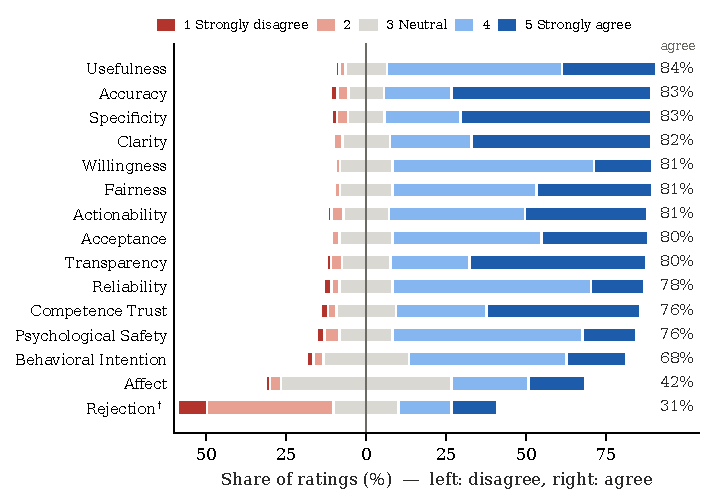
\includegraphics[width=0.74\textwidth]{figures/likert_items.pdf}
\Description{Diverging stacked bar chart of the fifteen items, sorted by percentage of agreement from Usefulness (84 percent) at the top to Affect (42 percent) and Rejection (31 percent) at the bottom. Disagreement segments to the left of zero are short for all items except Rejection; Affect has a large neutral segment.}
\caption{Distribution of ratings per item, sorted by the share of agreement (right-hand labels). Neutral ratings are centred on zero.}
\label{fig:likert}
\end{figure}

\paragraph{What drives acceptance.}
Table~\ref{tab:drivers} reports the mixed models of Eq.~\eqref{eq:drivers}. Perceived utility was the strongest predictor of acceptance and of continued-use intention: one standard deviation in utility corresponded to 0.30 points more acceptance and 0.28 points more intention. Trust added a similar amount to both outcomes (0.22 points each). Perceived quality contributed to acceptance (0.19 points) but not to willingness or intention once utility and trust were in the model. Willingness to revise followed a different pattern: it was driven mainly by affect (0.23 points), with a smaller contribution from utility (0.13 points). The fixed effects explained 61\% of the variance in acceptance, 39\% in willingness and 44\% in intention. Collinearity was moderate (maximum VIF 3.2).

\begin{table}[t]
\caption{Mixed models of acceptance, willingness to revise and behavioural intention (Eq.~\ref{eq:drivers}). Coefficients are rating points per SD of the predictor (SE). $^{*}p<.05$, $^{**}p<.01$, $^{***}p<.001$.}
\label{tab:drivers}
\centering\scriptsize
\setlength\tabcolsep{6pt}
\begin{tabular}{@{}lccc@{}}
\toprule
Predictor & Acceptance & Willingness & Behav.\ intention \\
\midrule
Perceived quality & 0.19 (0.05)$^{***}$ & 0.05 (0.05) & $-$0.02 (0.06) \\
Perceived utility & 0.30 (0.05)$^{***}$ & 0.13 (0.05)$^{**}$ & 0.28 (0.06)$^{***}$ \\
Trust & 0.22 (0.05)$^{***}$ & 0.10 (0.05) & 0.22 (0.06)$^{***}$ \\
Affect & $-$0.03 (0.04) & 0.23 (0.04)$^{***}$ & 0.14 (0.05)$^{**}$ \\
\midrule
Marginal / conditional $R^2$ & .61 / .66 & .39 / .53 & .44 / .59 \\
\bottomrule
\end{tabular}
\end{table}

\paragraph{Is acceptance self-serving?}
For the 171 instances with criterion scores (Rubric and Researching), students did not reward higher AI scores. If anything, acceptance ($\rho=-.15$, $p=.050$), fairness ($\rho=-.12$, $p=.10$) and the agreement index ($\rho=-.07$, $p=.35$) were slightly lower when the AI scored the answer higher.

\subsection{RQ2: Differences Between Feedback Formats}

\begin{table}[t]
\caption{Ratings by feedback format, mean (SD). Friedman tests over the 86 students, each of whom rated all four formats; $p$ for the construct rows is Holm-adjusted. Tokens: mean LLM input / output tokens per feedback instance (86 instances per format).}
\label{tab:rq2}
\centering\scriptsize
\setlength\tabcolsep{3pt}
\begin{tabular}{@{}lccccccc@{}}
\toprule
 & Sandwich & Rubric & Explainable & Researching & $\chi^2(3)$ & $p$ & $W$ \\
\midrule
% generated by analysis/run_analysis.py -> analysis/tables/rq2_formats.tex
Agreement index (AAI) & 4.12 (0.69) & 4.01 (0.66) & 4.07 (0.61) & 4.09 (0.60) & 23.04 & $<$.001 & 0.089 \\
\midrule
Perceived quality & 4.36 (0.82) & 4.33 (0.82) & 4.39 (0.79) & 4.28 (0.86) & 6.31 & .195 & 0.024 \\
Perceived utility & 4.27 (0.86) & 4.01 (0.69) & 3.95 (0.66) & 4.22 (0.73) & 45.57 & $<$.001 & 0.177 \\
Trust & 4.12 (0.78) & 3.91 (0.75) & 4.11 (0.70) & 4.12 (0.65) & 24.98 & $<$.001 & 0.097 \\
Affect & 3.74 (0.69) & 3.65 (0.75) & 3.63 (0.76) & 3.72 (0.68) & 10.22 & .050 & 0.040 \\
Acceptance \& intention & 3.95 (0.70) & 3.91 (0.71) & 3.96 (0.62) & 3.98 (0.62) & 3.70 & .295 & 0.014 \\
\midrule
Feedback length (words) & 248 & 267 & 215 & 623 & 172.19 & $<$.001 & 0.667 \\
Tokens/instance (in/out) & 10.0k/526 & 10.6k/617 & 12.0k/474 & 18.3k/2{,}113 & & & \\
\bottomrule
\end{tabular}
\end{table}

The four formats received similar but not identical ratings (Table~\ref{tab:rq2}, Fig.~\ref{fig:formats}). Mean agreement ranged from 4.01 (Rubric) to 4.12 (Sandwich). The Friedman test detected a difference ($\chi^2(3)=23.04$, $p<.001$), but its size was small ($W=.09$). Pairwise tests located it between Sandwich and the two formats without next steps: Sandwich was rated 0.11 points above Rubric ($p_\text{Holm}=.002$) and 0.06 points above Explainable ($p_\text{Holm}=.023$); no other pair differed after correction. The mixed model, which weighs the size of each difference rather than its rank, was less conclusive (likelihood-ratio $\chi^2(3)=6.65$, $p=.084$; Rubric vs.\ Sandwich $b=-0.11$, $p=.013$). Many students rated the formats almost alike but in a consistent order, which a rank test detects more easily.

The differences were concentrated in two constructs. Perceived utility varied most ($\chi^2(3)=45.57$, $p_\text{Holm}<.001$, $W=.18$): Sandwich (4.27) and Researching (4.22) were rated more useful and actionable than Rubric (4.01) and Explainable (3.95). At the item level this gap was largest for actionability (4.33 and 4.28 vs.\ 3.97 and 3.95; $p_\text{Holm}<.001$), which matches the one structural feature these two formats share: an explicit list of next steps. Trust also varied ($\chi^2(3)=24.98$, $p_\text{Holm}<.001$, $W=.10$), with Rubric lowest (3.91 vs.\ 4.11--4.12); Rubric feedback also received the lowest ratings for competence trust (3.97) and fairness (3.95), and fairness is the item that refers directly to a score. Sandwich feedback was rated highest on affect (3.69 vs.\ 3.41 for Explainable; item $p_\text{Holm}=.016$). Perceived quality and acceptance \& intention did not differ, and the \textsc{Acceptance} item itself was almost constant across formats (4.05--4.12, $p_\text{Holm}=1.00$). Researching feedback was rated somewhat less clear than the others (4.19 vs.\ 4.36--4.41), but this did not survive correction ($p_\text{Holm}=.22$).

Length does not explain the pattern: Researching feedback was about 2.5 times as long as the others ($\chi^2(3)=172.2$, $p<.001$, $W=.67$) yet rated on a par with Sandwich. It was also the costliest, at 20.4k tokens per instance versus 10.5k--12.5k for the other formats and four times Sandwich's output tokens; it used 37\% of the study's 4.70M tokens. Adding feedback length and answer length to the mixed model left the Rubric gap unchanged ($b=-0.11$, $p=.018$), and neither covariate was related to agreement (feedback length $b=-0.06$, $p=.16$; answer length $b=0.01$, $p=.78$).

For all six format pairs, the 90\% confidence interval of the paired difference in agreement fell inside $\pm0.25$ points; the most extreme bound was 0.21 (Sandwich vs.\ Rubric, interval $[0.02, 0.21]$). The result held without straight-lined responses (280 responses, 64 complete blocks; $\chi^2(3)=23.51$, $p<.001$, $W=.12$), with the same ordering.

One reason the effects are small is that most variance lay between students: the intraclass correlation of the agreement index was .77 (also .77 without straight-lined responses), leaving only a quarter of the variance within students for format to explain.

\begin{figure}[t]
\centering
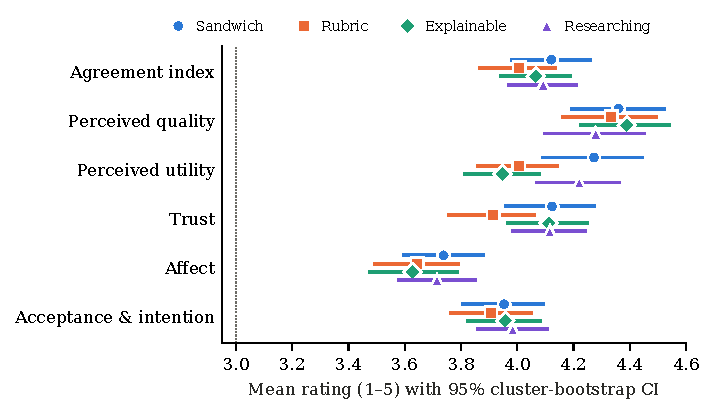
\includegraphics[width=0.68\textwidth]{figures/format_constructs.pdf}
\Description{Dot plot with confidence intervals of the agreement index and five construct scores for each of the four feedback formats. Most points lie between about 3.6 and 4.4. The intervals overlap heavily, except in perceived utility, where Sandwich and Researching sit to the right of Rubric and Explainable, and in trust, where Rubric sits to the left of the other three.}
\caption{Agreement index and construct scores by feedback format, with 95\% cluster-bootstrap confidence intervals. The dotted line marks the neutral midpoint.}
\label{fig:formats}
\end{figure}

\ifrqthree
\subsection{RQ3: Raw-Code versus Graph-Based Questions}
Raw-code and graph-based questions received similar agreement (Table~\ref{tab:rq3}; 4.14 vs.\ 4.06), and the mixed model, controlling for format and student, agreed ($b=0.08$, $SE=0.06$, $p=.22$, 95\% CI $[-0.04, 0.20]$). Much of this gap reflects who received raw-code questions: among the 26 students who answered both types, the two means were almost identical (3.99 raw vs.\ 4.01 graph). The largest construct difference was in perceived quality (4.52 vs.\ 4.30; Mann--Whitney $p=.021$, $p_\text{Holm}=.11$), driven by transparency (4.59 vs.\ 4.22; $p=.006$, $p_\text{Holm}=.10$). The direction is plausible, since raw-code feedback could quote the actual methods, but no difference survived correction. The confidence interval of the mixed model rules out a raw-code advantage larger than about 0.2 points and any meaningful advantage for graph-based questions.

\begin{table}[t]
\caption{Agreement by question context type, mean. $b$: mixed-model estimate for raw code vs.\ graph, controlling for format, with a random intercept per student.}
\label{tab:rq3}
\centering\scriptsize
\setlength\tabcolsep{5pt}
\begin{tabular}{@{}lcccccc@{}}
\toprule
Context & $n$ & AAI & Quality & Utility & Trust & Acceptance \& int. \\
\midrule
Graph & 280 & 4.06 & 4.30 & 4.11 & 4.05 & 3.94 \\
Raw code & 64 & 4.14 & 4.52 & 4.12 & 4.16 & 4.00 \\
\midrule
\multicolumn{7}{@{}l}{$b_\text{raw}=0.08$ ($SE=0.06$), $p=.22$; Mann--Whitney $p$ for AAI $=.22$} \\
\bottomrule
\end{tabular}
\end{table}
\fi

\subsection{Students' Free-Text Replies}
Optional free-text replies were left on 160 instances (46.5\%) by 44 students, mostly one or two sentences (median 35 words); we coded them with a simple keyword scheme, so the shares below are approximate. About three in five replies (59\%) named a concrete revision, typically by dropping a claim the feedback had shown to be unsupported (``I'll drop the idea that the record is deleted, since the flow has no delete step''). About half (53\%) asked a follow-up question about something the feedback left open, most often the exact error code or the step at which a check happens; many replies did both. Outright disagreement was rare but specific. One student showed that a validation function returns \texttt{409 SCHEDULE\_CONFIRMED} before the lock check and objected that the AI had ``guessed'' a different error name, a hallucination that code grounding should prevent; another pointed out that the feedback had confused the type of request the question was about. One reply concerned presentation: feedback written as a single block of text was ``very hard to read''.

%=============================================================================
\section{Discussion}
\label{sec:discussion}

\paragraph{Students accept the diagnosis more readily than they are moved by it.}
Students largely agreed that the feedback on their answers was accurate, specific and usable, and most also trusted the system's competence. Fewer committed to using it again, and most were neutral about whether it motivated them. The free-text replies read the same way: students corrected individual claims and asked precise follow-up questions---engaged, but businesslike. The replies also show students catching the occasional error, which is what calibrated trust~\cite{lee2004trust} asks of users of a tool that is usually, but not always, right.

\paragraph{Utility and trust matter more than correctness.}
Perceived utility and trust predicted acceptance and continued-use intention more strongly than perceived quality, as research on technology acceptance predicts~\cite{davis1989perceived,venkatesh2003user}; quality had no independent link to willingness or future use, and willingness depended mostly on affect. AI feedback should therefore be judged on whether students know what to do next and whether they feel like doing it, not only on whether its diagnosis is right.

\paragraph{What helps is next steps, not the format label.}
Within the same students, the four formats produced ratings that differed reliably but by less than a quarter of a scale point. They differed not in perceived quality or acceptance but in how useful and actionable students found them. The two formats rated highest, Sandwich and Researching, are the two that end with a list of next steps; Rubric and Explainable, which leave the student to infer what to change, were rated lower. Rubric feedback was also trusted less, perhaps because a visible score invites comparison with the student's own estimate. Two practical consequences follow. First, whatever the format, feedback should close with concrete next steps. Second, the two-model Researching pipeline produced 2.5 times as much text, used about twice the tokens of Sandwich and needed a second provider, yet was rated no higher than a single-model Sandwich and slightly less clear, so its cost is hard to justify on student agreement alone. The high intraclass correlation also means that between-group comparisons of feedback designs risk confounding format with student disposition; within-subject designs are safer.

\paragraph{Measuring agreement is harder than it looks.}
Almost a fifth of the responses were straight-lined, enough to blur the reverse-worded item in the full sample; long batteries of ratings invite this, and each student gave sixty~\cite{kim2019straightlining}. We recommend fewer items per instance (the subscales are internally consistent enough to shorten), an attention check or positively worded behavioural probes instead of reversed items~\cite{vansonderen2013ineffectiveness}, and provenance markers on every record so that non-research data can be excluded mechanically.

\paragraph{Threats to validity.}
\emph{Internal validity.} Format was randomised within students, which protects the RQ2 comparison against individual differences. The ratings in RQ1 are self-reports collected in a single instrument, so common-method variance may inflate the correlations among constructs~\cite{podsakoff2003common}, and the driver models are associational, not causal. \emph{Construct validity.} The instrument was developed for this study and has not undergone confirmatory factor analysis; the \textsc{Rejection} item worked only among attentive respondents, and the affect subscale had low reliability. We did not measure whether students actually revised their answers or whether the feedback was technically correct according to experts, so ``agreement'' should not be read as ``learning'' or ``accuracy''. Free-text coding was keyword-based. \emph{External validity.} The sample comes from one university, and a novelty effect may have inflated ratings. With 86 complete blocks the study can detect small-to-medium within-subject effects, and we report equivalence bounds so that significant but negligible differences are not overinterpreted. RQ3 is weaker: context type was assigned by the system rather than randomised, only 64 instances used raw-code questions, and the same context type also served as the evaluator's ground truth, so question source and feedback context are confounded. \emph{Statistical conclusion validity.} Likert ratings are ordinal; we used rank-based tests as the primary analyses and treated mixed models, which assume interval scaling, as confirmatory. For RQ2 the two disagreed at $p=.05$, another reason to read the format effects as small.

%=============================================================================
\section{Conclusion}
\label{sec:conclusion}

We studied how students in software project courses respond to LLM feedback on their answers to questions about their own team's code. Across 344 rated feedback instances from 86 students, agreement was positive (4.07 on a five-point scale): students accepted the diagnosis readily, but fewer intended to keep using the system and most were neutral about whether the feedback motivated them. Perceived utility and trust, more than perceived quality, were the strongest correlates of acceptance and of intention to keep using the system. The four feedback formats---Sandwich, Rubric, Explainable and a two-model Researching ensemble---differed only slightly, by at most a quarter of a scale point: formats with explicit next steps were rated more actionable, and Rubric feedback was trusted less. Most variance lay between students, and raw-code and graph-based questions were rated alike.

Future work will link feedback to students' later revisions and to expert judgements of its correctness. We also plan a shortened instrument with an attention check and without reverse-worded items, an experiment that adds next steps to every format, and a study that randomises the context type of each question so that raw-code and graph-based questions can be compared with balanced groups.

\begin{credits}
\subsubsection{\ackname}
% TODO: acknowledge course instructors, funding (if any), and participating students.
We thank the students and instructors of the participating software project courses.

\subsubsection{\discintname}
The authors have no competing interests to declare that are relevant to the content of this article.
% TODO: add an ethics/consent statement as required by the university (e.g., informed consent, anonymised data).
\end{credits}

\bibliographystyle{splncs04}
\bibliography{refs}

\end{document}
